\subsection{Ein bisschen Typografie}

\begin{frame}[fragile]{Schönere Brüche im Text}
  \begin{Packages}
    \begin{lstlisting}
      \usepackage{xfrac}
    \end{lstlisting}
  \end{Packages}
  \begin{itemize}
    \item Problem: \lstinline+\frac{1}{2}+ zu hoch
    \item unschöne Alternative: 1/2
    \item schön: \lstinline+\sfrac{1}{2}+
  \end{itemize}
  \begin{CodeExample}{0.5}
    \begin{lstlisting}
      \sfrac{1}{2}
      \sfrac{$\mathup{\pi}$}{2}
    \end{lstlisting}
  \CodeResult
    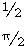
\includegraphics[scale=0.8]{figures/xfrac.pdf}
  \end{CodeExample}
\end{frame}

\begin{frame}[fragile]{Geschützte Leerzeichen}
  \begin{itemize}
    \item Es gibt Leerzeichen an denen nicht umgebrochen werden soll
    \item Zwischen Titel und Name
    \item Bei Referenzen
    \item zweiteilige Abkürzungen (aber ein kleines!)
    \item Bei Datumsangaben
    \item Zweiteilige Ortsnamen
    \item Zwischen Zahl und Einheit (→\texttt{siunitx})
  \end{itemize}
  \begin{CodeExample}{0.5}
    \begin{lstlisting}
      Prof.~Dr.~Dr.~Rhode
      Abbildung~\ref{fig:peplogo}
      z.\,B.
      2.~Oktober~2014
      St.~Helena
    \end{lstlisting}
    \CodeResult
      Prof.~Dr.~Dr.~Rhode \\
      Abbildung~\ref{fig:peplogo} \\
      z.\,B. \\
      2.~Oktober~2014 \\
      St.~Helena
  \end{CodeExample}
\end{frame}

\begin{frame}[fragile]{Striche}
  \begin{block}{Benötigte Einstellung}
    \begin{lstlisting}
      \defaultfontfeatures{Ligatures=TeX}
    \end{lstlisting}
  \end{block}
  Es gibt vier verschiedene Striche:
  \begin{CodeExample}{0.49}
    \begin{lstlisting}
      - $-$ -- ---
    \end{lstlisting}
  \CodeResult
    - $-$ -- ---
  \end{CodeExample}

  \begin{itemize}
    \item -- (en-dash) ist der Gedankenstrich (nicht für Protokolle)
      \begin{lstlisting}
        Text -- oh, Gedankenstriche -- Text
      \end{lstlisting}
    \item -- zwischen Namen von unterschiedlichen Personen
      \begin{lstlisting}
        Maxwell--Boltzmann-Verteilung
      \end{lstlisting}
    \item - zwischen Doppelnamen der selben Person
      \begin{lstlisting}
        Levi-Civita-Symbol
      \end{lstlisting}
    \item -- ist auch der Streckenstrich
      \begin{lstlisting}
        1 bis 10 ist 1--10
      \end{lstlisting}
    \item --- (em-dash) kommt im Deutschen nicht vor, ist aber der englische Gedankenstrich
      \begin{lstlisting}
        text---oh, em-dashes---text
      \end{lstlisting}
  \end{itemize}
\end{frame}

\begin{frame}[fragile]{
  Trennung bei Strichen \hfill
  \doc{http://mirrors.ctan.org/macros/latex/contrib/ncctools/doc/extdash.pdf}{extdash}
}
  \vspace*{-2em}
  \begin{Packages}
    \begin{lstlisting}
      \usepackage[shortcuts]{extdash} % nach hyperref, bookmark
    \end{lstlisting}
  \end{Packages}

  \LaTeX\ trennt Wörter nur an Strichen, falls welche da sind.\\
  So trennt man sie trotzdem:
  \vspace{-0.5em}
  \begin{CodeExample}{0.85}[Trennbare Striche]
    \begin{lstlisting}
      \-/ \-- \---
      Maxwell--Boltzmann-Verteilung
      Maxwell\--Boltzmann\-/Verteilung
    \end{lstlisting}
  \CodeResult
    - -- --- \\
    Maxwell--Boltzmann-Verteilung \\
    Maxwell\--Boltzmann\-/Verteilung
  \end{CodeExample}

  \vspace{-7em}
  So verhindert man die Trennung an den Strichen:
  \begin{lstlisting}
    \=/ \== \===
    $x$\=/Achse
  \end{lstlisting}
\end{frame}

\begin{frame}[fragile]{Silbentrennung}
  \begin{itemize}
    \item Manchmal kann \LaTeX\ ein Wort nicht richtig trennen
    \item Manche Fachwörter sollten nicht nach deutschen Regeln getennt werden
  \end{itemize}
  \begin{block}{Trennung für Wort vorgeben}
    \begin{lstlisting}
      % Präambel
      \hyphenation{Dia-mag-ne-tis-mus hy-phen-ate hy-phen-a-tion}
      % statt Di-a-mag-ne-tis-mus

      hy\-phen\-ate % im Text
    \end{lstlisting}
  \end{block}
\end{frame}
